\chapter{Algebras and Initial Algebras}
\label{chap:algebras}

\epigraph{
  ``Curiouser and curiouser!''
}{---\textcite[23]{carroll-2004}}

In this chapter we explore algebras and initial algebras over
endofunctors, and their relation to algebraic data types in Haskell.
As motivation, \texthaskell{foldr} is a standard function that
encapsulates common patterns of induction and recursion concerning
lists \parencite[355--356]{hutton-1999}. The \texthaskell{foldr}
function can be defined as follows\footnote{Note that this is not the
  type signature of the standard Haskell \texthaskell{foldr}
  function.}:
\begin{codehaskell}
foldr :: b -> (a -> b -> b) -> [a] -> b
foldr n c []     = n
foldr n c (x:xs) = c x (foldr n c xs)
\end{codehaskell}
That is, given a value \texthaskell{n} of type \texthaskell{b} and a
function \texthaskell{c} of type \texthaskell{a -> b -> b}, the
function \texthaskell{foldr n c} of type \texthaskell{[a] -> b}
replaces \texthaskell{[]} with \texthaskell{n} and \texthaskell{(:)}
with \texthaskell{c}. This amounts to saying that \texthaskell{[a]}
and its constructors, \texthaskell{[]} and \texthaskell{(:)}, yield an
algebra over an endofunctor, and, more important, that it constitutes
the initial algebra over the endofunctor. As it turns out, this fact
uniquely determines both the type signature and the definition of the
\texthaskell{foldr} function.

This idea generalizes to algebraic data types in the sense that one
such type is the initial algebra over an endofunctor and that this
fact uniquely determines a function that encapsulates common patterns
of induction and recursion concerning that type.

\section{Algebras and Initial Algebras}
\label{sec:algebras}

We begin by describing algebras (over endofunctors) and algebra
homomorphisms.

\begin{definition}
  \label{def:algebra}

  %% \parencite[15]{vene-2000}

  Let $\func{F}: \cat{C} \to \cat{C}$ be an endofunctor in a category
  $\cat{C}$. An \func{F}-al\-ge\-bra $(a,\alpha)$ is an object $a$,
  called the carrier of the algebra, and a morphism $\alpha:
  \funcO{F}(a) \to a$.

\end{definition}

As examples, we consider the initial object of a category, and natural
numbers and lists in \set, which we shall describe again as examples
of algebras in Haskell.

\begin{example}
  \label{ex:algebra-initial-object}

  %% \parencite[18]{vene-2000}

  Let \cat{C} be a category with an initial object $0$. Then
  $(0,\idO{0})$ is an algebra over the identity functor (see Example
  \ref{ex:functor-identity}), that is, an \func{I}-al\-ge\-bra. In
  particular, in \set, $(\emptyset,\idO{\emptyset})$ is an
  \func{I}-algebra.

\end{example}

\begin{example}
  \label{ex:algebra-natural}

  %% \parencite[18--19]{vene-2000}

  In \set, the natural numbers $\mathbb{N} = \{0,1,2,...\}$, along
  with the functions $\zero: 1 \to \mathbb{N}$ and $\suc: \mathbb{N}
  \to \mathbb{N}$, which can be joined to a function $[\zero,\suc]: 1
  + \mathbb{N} \to \mathbb{N}$, as illustrated by the diagram in
  Figure \ref{fig:coproduct-natural}, yield an algebra
  $(\mathbb{N},[\zero,\suc])$ over an endofunctor $\func{N}: \set \to
  \set$ whose object mapping assigns to each set $A$ a set
  \begin{equation*}
    \funcO{N}(A) = 1 + A
    \text{,}
  \end{equation*}
  and whose morphism mapping assigns to each function $f: A \to B$ a
  function $\funcM{N}(f): 1 + A \to 1 + B$ such that
  \begin{equation*}
    \funcM{N}(f) \comp \iota_{1} = \iota_{1}
    \quad
    \text{and}
    \quad
    \funcM{N}(f) \comp \iota_{2} = \iota_{2} \comp f
    \text{,}
  \end{equation*}
  that is,
  \begin{equation*}
    \funcM{N}(f)(1,()) = (1,())
    \quad
    \text{and}
    \quad
    \funcM{N}(f)(2,x) = (2,f(x))
  \end{equation*}
  for all $x \in A$ (see Examples
  \ref{ex:initial-terminal-objects-set} and \ref{ex:coproduct-set} for
  initial objects and coproducts in \set, respectively).

  \begin{figure}[htb]
    \begin{center}
      \begin{tikzpicture}[node distance=4cm]
        \node (ab)               {$1 + \mathbb{N}$};

        \node (a)  [left of=ab]  {$1$};
        \node (b)  [right of=ab] {$\mathbb{N}$};
        \node (c)  [below of=ab] {$\mathbb{N}$};

        \draw [<-] (ab) to node [swap] {$\iota_{1}$} (a);
        \draw [<-] (ab) to node        {$\iota_{2}$} (b);

        \draw [<-] (c)  to node        {$\zero$} (a);
        \draw [<-] (c)  to node [swap] {$\suc$} (b);

        \draw [<-,dotted] (c)  to node [swap] {$[\zero,\suc]$} (ab);
      \end{tikzpicture}
    \end{center}
    \caption{Natural numbers in \set.}
    \label{fig:coproduct-natural}
  \end{figure}

\end{example}

\begin{example}
  \label{ex:algebra-list}

  %% \parencite[19--20]{vene-2000}

  In \set, lists can be represented as algebras over endofunctors. For
  a given set $A$,
  \begin{equation*}
    \nil: 1 \to \listof{A}
    \quad
    \text{and}
    \quad
    \cons: A \times \listof{A} \to \listof{A}
  \end{equation*}
  can be joined to a function $[\nil,\cons]: 1 + A \times \listof{A}
  \to \listof{A}$, as illustrated by the diagram in Figure
  \ref{fig:coproduct-list}. In this way, $(\listof{A},[\nil,\cons])$
  is an algebra over an endofunctor $\func{L}^{A}: \set \to \set$
  whose object mapping assigns to each set $B$ a set
  \begin{equation*}
    \funcO{L}^{A}(B) = 1 + A \times B
    \text{,}
  \end{equation*}
  and whose morphism mapping assigns to each function $g: B \to C$ a
  function $\funcM{L}^{A}(g): 1 + A \times B \to 1 + A \times C$ such
  that
  \begin{equation*}
    \funcM{L}^{A}(g)(1,()) = (1,())
    \quad
    \text{and}
    \quad
    \funcM{L}^{A}(g)(2,(x,y)) = (2,(x,g(y)))
  \end{equation*}
  for all $(x,y) \in A \times B$ (see Examples
  \ref{ex:initial-terminal-objects-set}, \ref{ex:product-set}, and
  \ref{ex:coproduct-set} for initial objects, products, and coproducts
  in \set, respectively).

  \begin{figure}[htb]
    \begin{center}
      \begin{tikzpicture}[node distance=4cm]
        \node (ab)               {$1 + A \times \listof{A}$};

        \node (a)  [left of=ab]  {$1$};
        \node (b)  [right of=ab] {$A \times \listof{A}$};
        \node (c)  [below of=ab] {$\listof{A}$};

        \draw [<-] (ab) to node [swap] {$\iota_{1}$} (a);
        \draw [<-] (ab) to node        {$\iota_{2}$} (b);

        \draw [<-] (c)  to node        {$\nil$} (a);
        \draw [<-] (c)  to node [swap] {$\cons$} (b);

        \draw [<-,dotted] (c)  to node [swap] {$[\nil,\cons]$} (ab);
      \end{tikzpicture}
    \end{center}
    \caption{Lists in \set.}
    \label{fig:coproduct-list}
  \end{figure}

\end{example}

\begin{definition}
  \label{def:algebra-homomorphism}

  %% \parencite[15]{vene-2000}

  Let $\func{F}: \cat{C} \to \cat{C}$ be an endofunctor in a category
  $\cat{C}$. If $(a,\alpha)$ and $(b,\beta)$ are \func{F}-algebras, an
  \func{F}-algebra homomorphism $f: (a,\alpha) \to (b,\beta)$ is a
  morphism $f: a \to b$ in $\cat{C}$ such that
  \begin{equation}
    \label{eq:algebra-homomorphism}
    \beta \comp \funcM{F}(f) = f \comp \alpha
    \text{,}
  \end{equation}
  that is, the diagram in Figure \ref{fig:algebra-homomorphism} is
  commutative. In this case, we say that $\dom(f) = (a,\alpha)$ and
  $\cod(f) = (b,\beta)$.

  \begin{figure}[htb]
    \begin{center}
      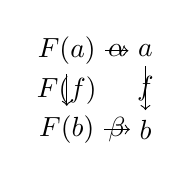
\begin{tikzpicture}
        \node (f a)                {$\funcO{F}(a)$};
        \node (a)   [right of=f a] {$a$};
        \node (f b) [below of=f a] {$\funcO{F}(b)$};
        \node (b)   [right of=f b] {$b$};

        \draw [->] (f a) to node        {$\alpha$} (a);
        \draw [->] (f b) to node [swap] {$\beta$}  (b);

        \draw [->] (a)   to node        {$f$}            (b);
        \draw [->] (f a) to node [swap] {$\funcM{F}(f)$} (f b);
      \end{tikzpicture}
    \end{center}
    \caption{An \func{F}-algebra homomorphism.}
    \label{fig:algebra-homomorphism}
  \end{figure}

\end{definition}

Let us now define identity and composite algebra homomorphisms, which
will allow us to construct categories of algebras and algebra
homomorphisms.

\begin{definition}
  \label{def:identity-algebra-homomorphism}

  Let $\func{F}: \cat{C} \to \cat{C}$ be an endofunctor in a category
  \cat{C}. If $(a,\alpha)$ is an \func{F}-algebra, then its identity
  \func{F}-algebra homomorphism
  \begin{equation*}
    \idO{(a,\alpha)}: (a,\alpha) \to (a,\alpha)
  \end{equation*}
  is the identity morphism $\idO{a}: a \to a$ in $\cat{C}$. To see
  that this is an \func{F}-al\-ge\-bra homomorphism, we prove
  \eqref{eq:algebra-homomorphism} with $f = \idO{(a,\alpha)}$:
  \begin{steps}
    \stepm{\alpha \comp \funcM{F}(\idO{a})}
      \eqby{\eqref{eq:functor-identity}}
    \stepm{\alpha \comp \idO{\funcO{F}(a)}}
      \eqby{\eqref{eq:category-identity} with $f = \alpha$}
    \stepm{\idO{a} \comp \alpha}
  \end{steps}

\end{definition}

\begin{definition}
  \label{def:composite-algebra-homomorphism}

  Let $\func{F}: \cat{C} \to \cat{C}$ be an endofunctor in a category
  \cat{C}, and $(a,\alpha)$, $(b,\beta)$, and $(c,\gamma)$ three
  \func{F}-algebras. Given two \func{F}-algebra homomorphisms, their
  composite \func{F}-algebra homomorphism $g \comp f: (a,\alpha) \to
  (c,\gamma)$ is the composite morphism $g \comp f: a \to c$ in
  $\cat{C}$. To see that this is an \func{F}-algebra homomorphism, we
  prove \eqref{eq:algebra-homomorphism} with $f = g \comp f$:
  \begin{steps}
    \stepm{\gamma \comp \funcM{F}(g \comp f)}
      \eqby{\eqref{eq:functor-composition}}
    \stepm{\gamma \comp \funcM{F}(g) \comp \funcM{F}(f)}
      \eqby{\eqref{eq:algebra-homomorphism} with $f = g$}
    \stepm{g \comp \beta \comp \funcM{F}(f)}
      \eqby{\eqref{eq:algebra-homomorphism}}
    \stepm{g \comp f \comp \alpha}
  \end{steps}

\end{definition}

\begin{definition}
  \label{def:category-alg}

  %% \parencite[16]{vene-2000}

  Let $\func{F}: \cat{C} \to \cat{C}$ be an endofunctor in a category
  \cat{C}. Then \func{F}-\alg is the category of \func{F}-algebras and
  \func{F}-algebra homomorphisms. Its objects are \func{F}-algebras,
  its morphisms are \func{F}-algebra homomorphisms, its identity
  morphisms are identity \func{F}-algebra homomorphisms, and its
  composite morphisms are composite \func{F}-algebra homomorphisms.
  Since \eqref{eq:category-associativity} and
  \eqref{eq:category-identity} hold for \cat{C}, they hold for
  \func{F}-\alg too.

\end{definition}

Having constructed categories of algebras and algebra homomorphisms,
we move on to their initial objects (see Definition
\ref{def:initial-object}), that is, initial algebras.

\begin{definition}
  \label{def:initial-algebra}

  %% \parencite[16]{vene-2000}

  Let $\func{F}: \cat{C} \to \cat{C}$ be an endofunctor in a category
  \cat{C}. An \func{F}-algebra $(\mu\func{F},\inmo)$ is the initial
  \func{F}-algebra of the category \func{F}-\alg if, for all
  \text{\func{F}-al}\-ge\-bras $(a,\alpha)$, there is a unique
  \func{F}-algebra homomorphism
  \begin{equation*}
    \cata\alpha: (\mu\func{F},\inmo) \to (a,\alpha)
    \text{,}
  \end{equation*}
  that is, a morphism $\cata\alpha: \mu\func{F} \to a$ in $\cat{C}$
  such that
  \begin{equation}
    \label{eq:cata-charn}
    \alpha \comp \funcM{F}(\cata\alpha) = \cata\alpha \comp \inmo
    \text{,}
  \end{equation}
  or, equivalently, the diagram in Figure \ref{fig:cata-charn} is
  commutative. Such an \func{F}-al\-ge\-bra homomorphism (that is, a
  unique \func{F}-algebra homomorphism from the initial
  \func{F}-algebra) is called a catamorphism.

  \begin{figure}[htb]
    \begin{center}
      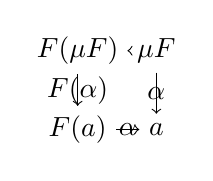
\begin{tikzpicture}
        \node (f a)                {$\funcO{F}(\mu\func{F})$};
        \node (a)   [right of=f a] {$\mu\func{F}$};
        \node (f b) [below of=f a] {$\funcO{F}(a)$};
        \node (b)   [right of=f b] {$a$};

        \draw [->] (f a) to node        {$\inmo$} (a);
        \draw [->] (f b) to node [swap] {$\alpha$}  (b);

        \draw [->] (a)   to node        {$\cata\alpha$}            (b);
        \draw [->] (f a) to node [swap] {$\funcM{F}(\cata\alpha)$} (f b);
      \end{tikzpicture}
    \end{center}
    \caption{A catamorphism.}
    \label{fig:cata-charn}
  \end{figure}

\end{definition}

Intuitively, the initial algebra denotes the collection of constructor
functions for inductive data types. This statement is justified by a
theorem, which we shall describe and prove using the following lemma.

\begin{lemma}
  \label{lem:cata-refl-fusion}

  %% \parencite[17]{vene-2000}

  Let $\func{F}: \cat{C} \to \cat{C}$ be an endofunctor in a category
  \cat{C}. If $(\mu\func{F},\inmo)$ is the initial \func{F}-algebra of
  the category \func{F}-\alg, then
  \begin{equation}
    \label{eq:cata-refl}
    \idO{\mu\func{F}} = \cata\inmo
  \end{equation}
  and, for all \func{F}-algebra homomorphisms $f: (a,\alpha) \to
  (b,\beta)$,
  \begin{equation}
    \label{eq:cata-fusion}
    f \comp \cata\alpha = \cata\beta
    \text{.}
  \end{equation}

  \begin{proof}

    Since $(\mu\func{F},\inmo)$ is initial, then $\cata\inmo$ and
    $\cata\beta$ are unique, which proves both equations. (For
    \eqref{eq:cata-fusion}, see the diagram in Figure
    \ref{fig:cata-fusion}.)

    \begin{figure}[htb]
      \begin{center}
        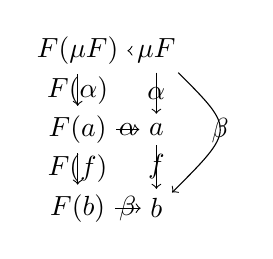
\begin{tikzpicture}
          \node (muf)                  {$\mu\func{F}$};
          \node (f muf) [left of=muf]  {$\funcO{F}(\mu\func{F})$};

          \node (a)     [below of=muf] {$a$};
          \node (f a)   [left of=a]    {$\funcO{F}(a)$};

          \node (b)     [below of=a]   {$b$};
          \node (f b)   [left of=b]    {$\funcO{F}(b)$};

          \node (c)     [right of=a]   {};

          \draw [->] (f muf) to node        {$\inmo$}  (muf);
          \draw [->] (f a)   to node [swap] {$\alpha$} (a);
          \draw [->] (f b)   to node [swap] {$\beta$}  (b);

          \draw [->] (muf) to node {$\cata\alpha$} (a);
          \draw [->] (a)   to node {$f$}           (b);

          \draw [->] (muf) .. controls (c) .. node {$\cata\beta$} (b);

          \draw [->] (f muf) to node [swap] {$\funcM{F}(\cata\alpha)$} (f a);
          \draw [->] (f a)   to node [swap] {$\funcM{F}(f)$}           (f b);
        \end{tikzpicture}
      \end{center}
      \caption{The fusion law for a catamorphism.}
      \label{fig:cata-fusion}
    \end{figure}

  \end{proof}

\end{lemma}

The following theorem is ``the formal justification on the
identification of inductive types with initial algebras''
\parencite[17]{vene-2000}.

\begin{theorem}
  \label{the:lambek}

  %% \parencite[17--18]{vene-2000}

  Let $\func{F}: \cat{C} \to \cat{C}$ be an endofunctor in a category
  \cat{C}. If $(\mu\func{F},\inmo)$ is the initial \func{F}-algebra of
  the category \func{F}-\alg, then $\inmo$ is an isomorphism with its
  inverse $\inmo^{-1}: \mu\func{F} \to \funcO{F}(\mu\func{F})$ defined
  by
  \begin{equation}
    \label{eq:lambek}
    \inmo^{-1} = \cata{\funcM{F}(\inmo)}
    \text{.}
  \end{equation}

  \begin{proof}

    We prove \eqref{eq:isomorphism} with $f = \inmo$. In the first
    place:
    \begin{steps}
      \stepm{\inmo \comp \inmo^{-1}}
        \eqby{\eqref{eq:lambek}}
      \stepm{\inmo \comp \cata{\funcM{F}(\inmo)}}
        \eqby{\eqref{eq:cata-fusion} with $f = \inmo$}
      \stepm{\cata\inmo}
        \eqby{\eqref{eq:cata-refl}}
      \stepm{\idO{\mu\func{F}}}
    \end{steps}
    In the second place:
    \begin{steps}
      \stepm{\inmo^{-1} \comp \inmo}
        \eqby{\eqref{eq:lambek}}
      \stepm{\cata{\funcM{F}(\inmo)} \comp \inmo}
        \eqby{\eqref{eq:cata-charn} with $\alpha = \funcM{F}(\inmo)$}
      \stepm{\funcM{F}(\inmo) \comp \funcM{F}(\cata{\funcM{F}(\inmo)})}
        \eqby{\eqref{eq:functor-composition} with $f = \cata{\funcM{F}(\inmo)}$ and $g = \inmo$}
      \stepm{\funcM{F}(\inmo \comp \cata{\funcM{F}(\inmo)})}
        \eqtext{see above}
      \stepm{\funcM{F}(\idO{\mu\func{F}})}
        \eqby{\eqref{eq:functor-identity} with $a = \mu\func{F}$}
      \stepm{\idO{\funcO{F}(\mu\func{F})}}
    \end{steps}

  \end{proof}

\end{theorem}

This ``theorem shows that the carrier of the initial algebra is (up to
isomorphism) a fixed point of the functor'' \parencite[18]{vene-2000}.
We have already discussed three examples of algebras (the initial
object of a category, natural numbers, and lists). We describe them
again as initial algebras.

\begin{example}
  \label{ex:initial-algebra-initial-object}

  %% \parencite[18]{vene-2000}

  Let \cat{C} be a category with an initial object $0$. Then
  $(0,\idO{0})$, the \func{I}-algebra described in Example
  \ref{ex:algebra-initial-object}, is the initial \func{I}-algebra of
  the category \func{I}-\alg. Indeed, given an \func{I}-algebra
  $(a,\alpha)$, there is a unique \func{I}-algebra homomorphism
  $\cata{\alpha}: (0,\idO{0}) \to (a,\alpha)$ in which the underlying
  morphism $\cata{\alpha}: 0 \to a$ in $\cat{C}$ is the unique
  morphism given by the fact that $0$ is an initial object. The
  uniqueness of this morphism guarantees that
  \eqref{eq:algebra-homomorphism} holds. In particular, in \set,
  $(\emptyset,\idO{\emptyset})$ is the initial \func{I}-algebra of the
  category \func{I}-\alg.

\end{example}

\begin{example}
  \label{ex:initial-algebra-natural}

  %% \parencite[18--19]{vene-2000}

  In \set, the \func{N}-algebra $(\mathbb{N},[\zero,\suc])$ described
  in Example \ref{ex:algebra-natural} is the initial \func{N}-algebra
  of the category \func{N}-\alg. For an \func{N}-algebra $(A,[z,s])$,
  that is, a set $A$ and functions $z: 1 \to A$ and $s: A \to A$, we
  need a unique \func{N}-algebra homomorphism $\cata{[z,s]}$ or
  \begin{equation*}
    \fold(z,s): (\mathbb{N},[\zero,\suc]) \to (A,[z,s])
    \text{,}
  \end{equation*}
  that is, a function $\fold(z,s): \mathbb{N} \to A$ such that
  \begin{equation*}
    \fold(z,s) \comp [\zero,\suc] = [z,s] \comp \funcM{N}(\fold(z,s))
    \text{.}
  \end{equation*}
  Without going into detail, this equation uniquely defines
  $\fold(z,s)$ as
  \begin{equation*}
    \fold(z,s)(\zero()) = z()
  \end{equation*}
  and, for all $n \in \mathbb{N}$,
  \begin{equation*}
    \fold(z,s)(\suc(n)) = s(\fold(z,s)(n))
    \text{,}
  \end{equation*}
  or, more succinctly,
  \begin{equation*}
    \fold(z,s)(n) = s^{n}(z())
    \text{,}
  \end{equation*}
  which yields the required unique \func{N}-algebra homomorphism.

  For instance, addition and multiplication of natural numbers can be
  defined as folds $\add$ and $\mul: \mathbb{N} \times \mathbb{N} \to
  \mathbb{N}$ such that, for all $(m,n) \in \mathbb{N} \times
  \mathbb{N}$,
  \begin{equation*}
    \add(m,n) = \fold(\lambda x.n,\suc)(m)
  \end{equation*}
  and
  \begin{equation*}
    \mul(m,n) = \fold(\zero,\lambda x.\add(m,x))(m)
    \text{,}
  \end{equation*}
  respectively.

\end{example}

\begin{example}
  \label{ex:initial-algebra-list}

  %% \parencite[19--20]{vene-2000}

  In \set, for a set $A$, the $\func{L}^{A}$-algebra
  $(\listof{A},[\nil,\cons])$ described in Example
  \ref{ex:algebra-list} is the initial algebra of the category
  $\func{L}^{A}$-\alg. Let $(B,[n,c])$ be an algebra over
  $\func{L}^{A}$, that is, a set $A$ and functions $n: 1 \to B$ and
  $c: A \times B \to B$. Then we need a unique $\func{L}^{A}$-algebra
  homomorphism $\fold(n,c): (\listof{A},[\nil,\cons]) \to (B,[n,c])$,
  that is, a function $\foldr(n,c): \listof{A} \to B$ such that
  \begin{equation*}
    \foldr(n,c) \comp [\nil,\cons] = [n,c] \comp \funcM{L}^{A}(\foldr(n,c))
    \text{.}
  \end{equation*}
  This equation uniquely defines $\fold(n,c)$ as
  \begin{equation*}
    \foldr(n,c)(\nil()) = n()
  \end{equation*}
  and, for all $(x,xs) \in A \times \listof{A}$,
  \begin{equation*}
    \foldr(n,c)(\cons(x,xs)) = c(x,\foldr(n,c)(xs))
    \text{,}
  \end{equation*}
  which yields the required unique $\func{L}^{A}$-algebra
  homomorphism.

  As an example, the length of a list of elements of a set $A$ can be
  calculated as a fold $\length: \listof{A} \to \mathbb{N}$ such that
  \begin{equation*}
    \length = \foldr(\zero,\lambda(x,n).\suc(n))
    \text{.}
  \end{equation*}
  As another example, two lists of elements of a set $A$ can be
  appended by a fold $\append: \listof{A} \times \listof{A} \to
  \listof{A}$ such that
  \begin{equation*}
    \append(xs,ys) = \foldr(\lambda x.ys,\cons)(xs)
  \end{equation*}
  for all $(xs,ys) \in \listof{A} \times \listof{A}$. Finally,
  $\map(f): \listof{A} \to \listof{B}$ can be defined as a fold
  \begin{equation*}
    \map(f) = \foldr(\nil,\lambda(x,ys).\cons(f(x),ys))
  \end{equation*}
  for all functions $f: A \to B$.

\end{example}

\section{Algebras and Initial Algebras in Haskell}
\label{sec:algebras-haskell}

In Haskell, when we define an algebraic data type, its declaration
introduces a new type or type constructor, and zero or more data
constructors. These data specify an initial algebra over an
endofunctor which can be inferred from the information at hand. Given
an algebraic data type, inferring such an endofunctor and proving that
its category of algebras has an initial object amounts to defining a
fold function for that particular type. In fact, such a function is
uniquely determined by the fact that the algebraic data type is an
initial algebra.

\begin{example}
  \label{ex:algebra-natural-haskell}

  %% We begin by describing natural numbers in Haskell in a similar way
  %% to that of Examples \ref{ex:algebra-natural} and
  %% \ref{ex:initial-algebra-natural}, that is, natural numbers in \set.

  In Haskell, natural numbers can be defined as an algebraic data
  type, as follows:
  \begin{codehaskell}
data Nat = Zero | Succ Nat
  \end{codehaskell}
  This declaration introduces a type \texthaskell{Nat} of kind
  \texthaskell{*}, and constructors \texthaskell{Zero} and
  \texthaskell{Succ} with types
  \begin{equation*}
    \text{\texthaskell{Zero :: Nat}}
    \quad
    \text{and}
    \quad
    \text{\texthaskell{Succ :: Nat -> Nat}}
    \text{.}
  \end{equation*}
  These data define an algebra over an endofunctor \texthaskell{N}:
  \begin{codehaskell}
data N a = Z | S a

instance Functor N where
  fmap _ Z     = Z
  fmap f (S x) = S (f x)
\end{codehaskell}
  In detail, this algebra is given by \texthaskell{Nat},
  \texthaskell{Zero}, and \texthaskell{Succ}. Moreover, the algebra in
  question is the initial algebra of the category of algebras over
  \texthaskell{N}:
  \begin{codehaskell}
fold :: a -> (a -> a) -> Nat -> a
fold z s Zero     = z
fold z s (Succ n) = s (fold z s n)
  \end{codehaskell}
  In words, given an algebra over \texthaskell{N}, that is, a type
  \texthaskell{a}, a value \texthaskell{z} of type \texthaskell{a},
  and a function \texthaskell{s} of type \texthaskell{a -> a}, there
  is a unique function of type \texthaskell{Nat -> a}, namely
  \texthaskell{fold z s}.

  For instance, given values \texthaskell{m} and \texthaskell{n} of
  type \texthaskell{Nat}, we define the addition of \texthaskell{m}
  and \texthaskell{n} using \texthaskell{fold n Succ}, that is,
  \texthaskell{fold} for the \texthaskell{N}-algebra specified by
  \texthaskell{Nat}, \texthaskell{n}, and \texthaskell{Succ}, as
  follows:
  \begin{codehaskell}
add :: Nat -> Nat -> Nat
add m n = fold n Succ m
  \end{codehaskell}
  This definition might be easier to understand if we compare it to
  the one yielded by using explicit recursion:
  \begin{codehaskell}
add Zero     n = n
add (Succ m) n = Succ (add m n)
  \end{codehaskell}

  As another example, given values \texthaskell{m} and \texthaskell{n}
  of type \texthaskell{Nat}, we define the multiplication of
  \texthaskell{m} and \texthaskell{n} using \texthaskell{fold Zero
    (add n)}, that is, \texthaskell{fold} for the
  \texthaskell{N}-algebra specified by \texthaskell{Nat},
  \texthaskell{Zero}, and \texthaskell{add n}, as follows:
  \begin{codehaskell}
mult :: Nat -> Nat -> Nat
mult m n = fold Zero (add n) m
  \end{codehaskell}
  In this case, explicit recursion yields the following definition:
  \begin{codehaskell}
mult Zero     n = Zero
mult (Succ m) n = add n (mul m n)
  \end{codehaskell}

\end{example}

Alternatively, we can consider \texthaskell{Nat} and
\begin{equation*}
  \text{\texthaskell{either (\textbackslash () -> Zero) Succ :: Either () Nat -> Nat}}
\end{equation*}
as an algebra over \texthaskell{Either ()} (see Example
\ref{ex:functor-coproduct-haskell}). So, given a type \texthaskell{b}
and
\begin{equation*}
  \text{\texthaskell{either (\textbackslash () -> z) s :: Either () a -> a}}
\end{equation*}
we need a unique function \texthaskell{fold} such that
\begin{equation*}
  \text{\texthaskell{fold z s . either (\textbackslash () -> Zero) Succ}}
\end{equation*}
and
\begin{equation*}
  \text{\texthaskell{either (\textbackslash () -> z) s . fmap (fold z s)}}
\end{equation*}
are the same, but that is the above definition of \texthaskell{fold}.

\begin{example}
  \label{ex:algebra-list-haskell}

  %% We now describe lists in Haskell in a similar way to that of
  %% Examples \ref{ex:algebra-list} and \ref{ex:initial-algebra-list},
  %% that is, lists in \set.

  In Haskell, lists can be defined as an algebraic data type, as
  follows:
  \begin{codehaskell}
data List a = Nil | Cons a (List a)
  \end{codehaskell}
  This declaration introduces a type constructor \texthaskell{List} of
  kind \texthaskell{* -> *}, and constructors \texthaskell{Nil} and
  \texthaskell{Cons} with types
  \begin{equation*}
    \text{\texthaskell{Nil :: List a}}
    \quad
    \text{and}
    \quad
    \text{\texthaskell{Cons :: a -> List a -> List a}}
  \end{equation*}
  for all types \texthaskell{a} of kind \texthaskell{*}. These data
  define an \texthaskell{L}-algebra:
  \begin{codehaskell}
data L a b = N | C a b

instance Functor (L a) where
  fmap _ N       = N
  fmap f (C x y) = C x (f y)
\end{codehaskell}
  More precisely, given a concrete type \texthaskell{a},
  \texthaskell{List a}, \texthaskell{Nil}, and \texthaskell{Cons}
  specify the algebra being discussed. This algebra is the initial
  algebra of the category of algebras over \texthaskell{L}:
  \begin{codehaskell}
foldr :: b -> (a -> b -> b) -> List a -> b
foldr n c Nil         = n
foldr n c (Cons x xs) = c x (foldr n c xs)
  \end{codehaskell}
  That is to say, for a concrete type \texthaskell{a}, given an
  algebra over \texthaskell{L}, that is, a concrete type
  \texthaskell{b}, a value \texthaskell{n} of type \texthaskell{b},
  and a function \texthaskell{c} of type \texthaskell{a -> b -> b},
  there is a unique function of type \texthaskell{List a -> b}, namely
  \texthaskell{foldr n c}.

  As an example, the length of a list of values of a type
  \texthaskell{a} can be calculated using \texthaskell{foldr}, as
  follows:
  \begin{codehaskell}
length :: List a -> Nat
length = foldr Zero (\_ -> Succ)
  \end{codehaskell}
  As another example, two lists \texthaskell{xs} and \texthaskell{ys}
  of values of a type \texthaskell{a} can be appended using
  \texthaskell{fold} for the \texthaskell{L}-algebra specified by
  \texthaskell{List a}, \texthaskell{ys}, and \texthaskell{Cons}:
  \begin{codehaskell}
append :: List a -> List a -> List a
append xs ys = (foldr ys Cons) xs
  \end{codehaskell}
  Finally, given concrete types \texthaskell{a} and \texthaskell{b},
  \texthaskell{map f} can be defined as a \texthaskell{foldr} for all
  functions \texthaskell{f} of type \texthaskell{a -> b}, as follows:
  \begin{codehaskell}
map :: (a -> b) -> List a -> List b
map f = foldr Nil (Cons . f)
  \end{codehaskell}
  Each of these definitions might be easier to understand if we
  compare them to the ones yielded by using explicit recursion:
  \begin{codehaskell}
length Nil         = Zero
length (Cons _ xs) = Succ (length xs)

append Nil         ys = ys
append (Cons x xs) ys = Cons x (concat xs ys)

map _ Nil         = Nil
map f (Cons x xs) = Cons (f x) (fmap f xs)
  \end{codehaskell}

\end{example}

\section{References}
\label{sec:algebras-references}

This chapter is based on \parencites[§
  10.5]{awodey-2010}[§~2.6]{bird-demoor-1997}[§ 2.1]{vene-2000}. The
definition of algebras over endofunctors, which is a simpler
description of algebras over monads, is also based on
\parencites[140]{maclane-1998}[595--596]{poigne-1992}.

\clearemptydoublepage
